\documentclass[]{final_report}
\usepackage{graphicx}
\usepackage{hyperref}
\usepackage[final]{pdfpages}


%%%%%%%%%%%%%%%%%%%%%%
%%% Input project details
\def\studentname{James King}
\def\reportyear{2018}
\def\projecttitle{Cooperative Strategies in Multi-Agent Systems}
\def\supervisorname{Kostas Stathis}
\def\degree{BSc (Hons) in Computer Science}
\def\fullOrHalfUnit{Full Unit} % indicate if you are doing the project as a Full Unit or Half Unit
\def\finalOrInterim{Interim Report} % indicate if this document is your Final Report or Interim Report

\begin{document}

\maketitle

%%%%%%%%%%%%%%%%%%%%%%
%%% Declaration

\chapter*{Declaration}

This report has been prepared on the basis of my own work. Where other published and unpublished source materials have been used, these have been acknowledged.

\vskip3em

Word Count: 

\vskip3em

Student Name: \studentname

\vskip3em

Date of Submission: 

\vskip3em

Signature:

\newpage

%%%%%%%%%%%%%%%%%%%%%%
%%% Table of Contents
\tableofcontents\pdfbookmark[0]{Table of Contents}{toc}\newpage

%%%%%%%%%%%%%%%%%%%%%%
%%% Your Abstract here

\begin{abstract}

\end{abstract}
\newpage

\chapter{Aims, Objectives and Literature Survey}

\section{Project Specification}
I will explore indirect reciprocity, by both researching and reporting on Nowak and other authors research on the mechanism, drawing on their research and possibly adding on to the ideas of onlookers and gossip to create a model for implementation. I shall be using the Axelrod-Python library to create a proof of concept that I am able to create a web application that allows users to set up and run games and tournaments. This web application will be hosted on Heroku and created using Flask and Python.\\\\
The solution that we are exploring for the interfacing issues between Python and Prolog is to create a web service for the agent's decision-making component. This will have a Prolog server containing what~\cite{prosocs} refers to as ``agent's minds". A mind will represent information on the state of the environment using an efficient version of the Event Calculus reported in~\cite{mvfcec}. Percepts can be added to the agent's mind and based on these percepts an agent will be able to decide on an action and act on it by returning an action to the environment. Separating out the head and body as in Stathis \textit{et al.} 2002~\cite{prosocs}, though this solution would take this separation further, having the head based in the Prolog service and the body in the environment (Python web application).\\\\
The capabilities of the Prolog service are to be demonstrated on the web application, which will run indirect reciprocity tournaments creating the environment that agents reside in and containing the body of the agent. The web application will use the service to input percepts and get actions.\\\\
These have been the core parts of the project however, I could extend this to the other mechanisms presented by Nowak~\cite{five_rules_coop} if I have time. Axelrod-Python has an implementation for network reciprocity - which would be interesting to use so I could create an especially nice frontend for the patterns created in the population~\cite{spatial}. Due to the nature of group selection working on top of direct reciprocity~\cite{multilevel_nowak} it would be possible to implement it on top of the Axelrod-Python library. Leaving kin selection to implement using the Prolog service.

\section{Aims and Objectives}
\begin{itemize}
\item To create a Prolog service that is able to support the decisions of a game-theoretic agent which interacts with other systems that wish to choose an agent, provide percepts from an environment and get actions from the agent.
\item To explore in a game-theoretic context a mechanism to aid in the evolution of cooperation known as indirect reciprocity.
\item To create a web application that allows users to set up and run game-theory tournaments of both direct and indirect reciprocity.
\item To use the web application to demonstrate an environment that combines the Prolog service and a set of game-theory strategies and evaluate the results.
\end{itemize}

\section{Literature Survey}
Description and critique of past work in relation to my project.

\chapter{Planning and Timescale}
Provide timeline of completed work and an updated one for next term.

\chapter{Summary of Completed Work}
Agents service, flask web app, environment, two reports

\section{Practical}

\subsection{Learning Web Dev}
Refer to Flask web.

\subsection{System Design}
Overall system design.

\subsection{Agents Service and API Design}
RESTful API. MVFCEC. Agent Template. Prolog service learning.

\subsection{Environment Design}

\subsection{Tools, Techniques and Processes}

TDD, UML, Processes in VCS, Testing Strategy

\section{Theory}
Summary of the reports and theory work.

%%%% ADD YOUR BIBLIOGRAPHY HERE
\newpage
\bibliography{../../refs.bib}{}
\bibliographystyle{plain}
\addcontentsline{toc}{chapter}{Bibliography}
\footnote{A lot of my background theory work has been completed in my earlier reports so many of the references appear in those reports (see appendix)}
\label{endpage}

\chapter{Appendix}
Introduce the two reports

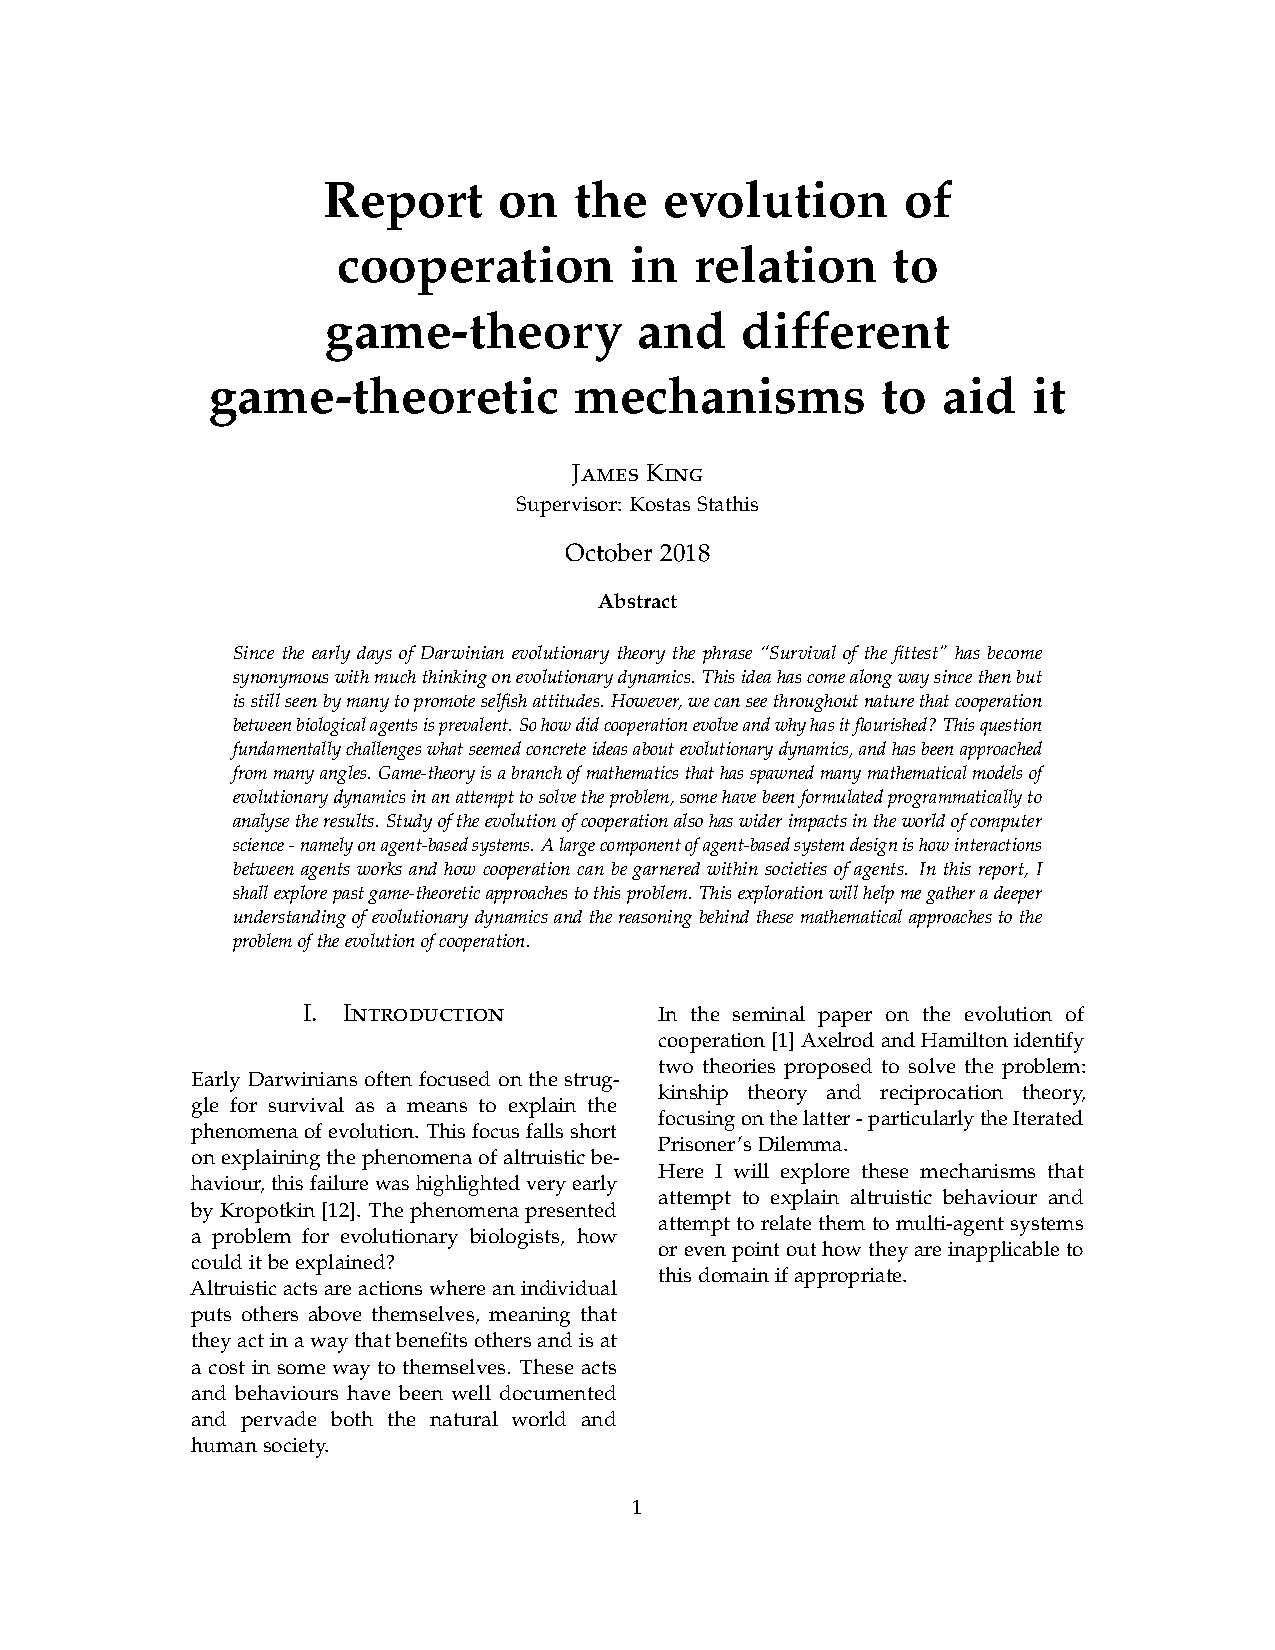
\includepdf[pages=-]{../../EvolCoop/EvolCoopReport.pdf}

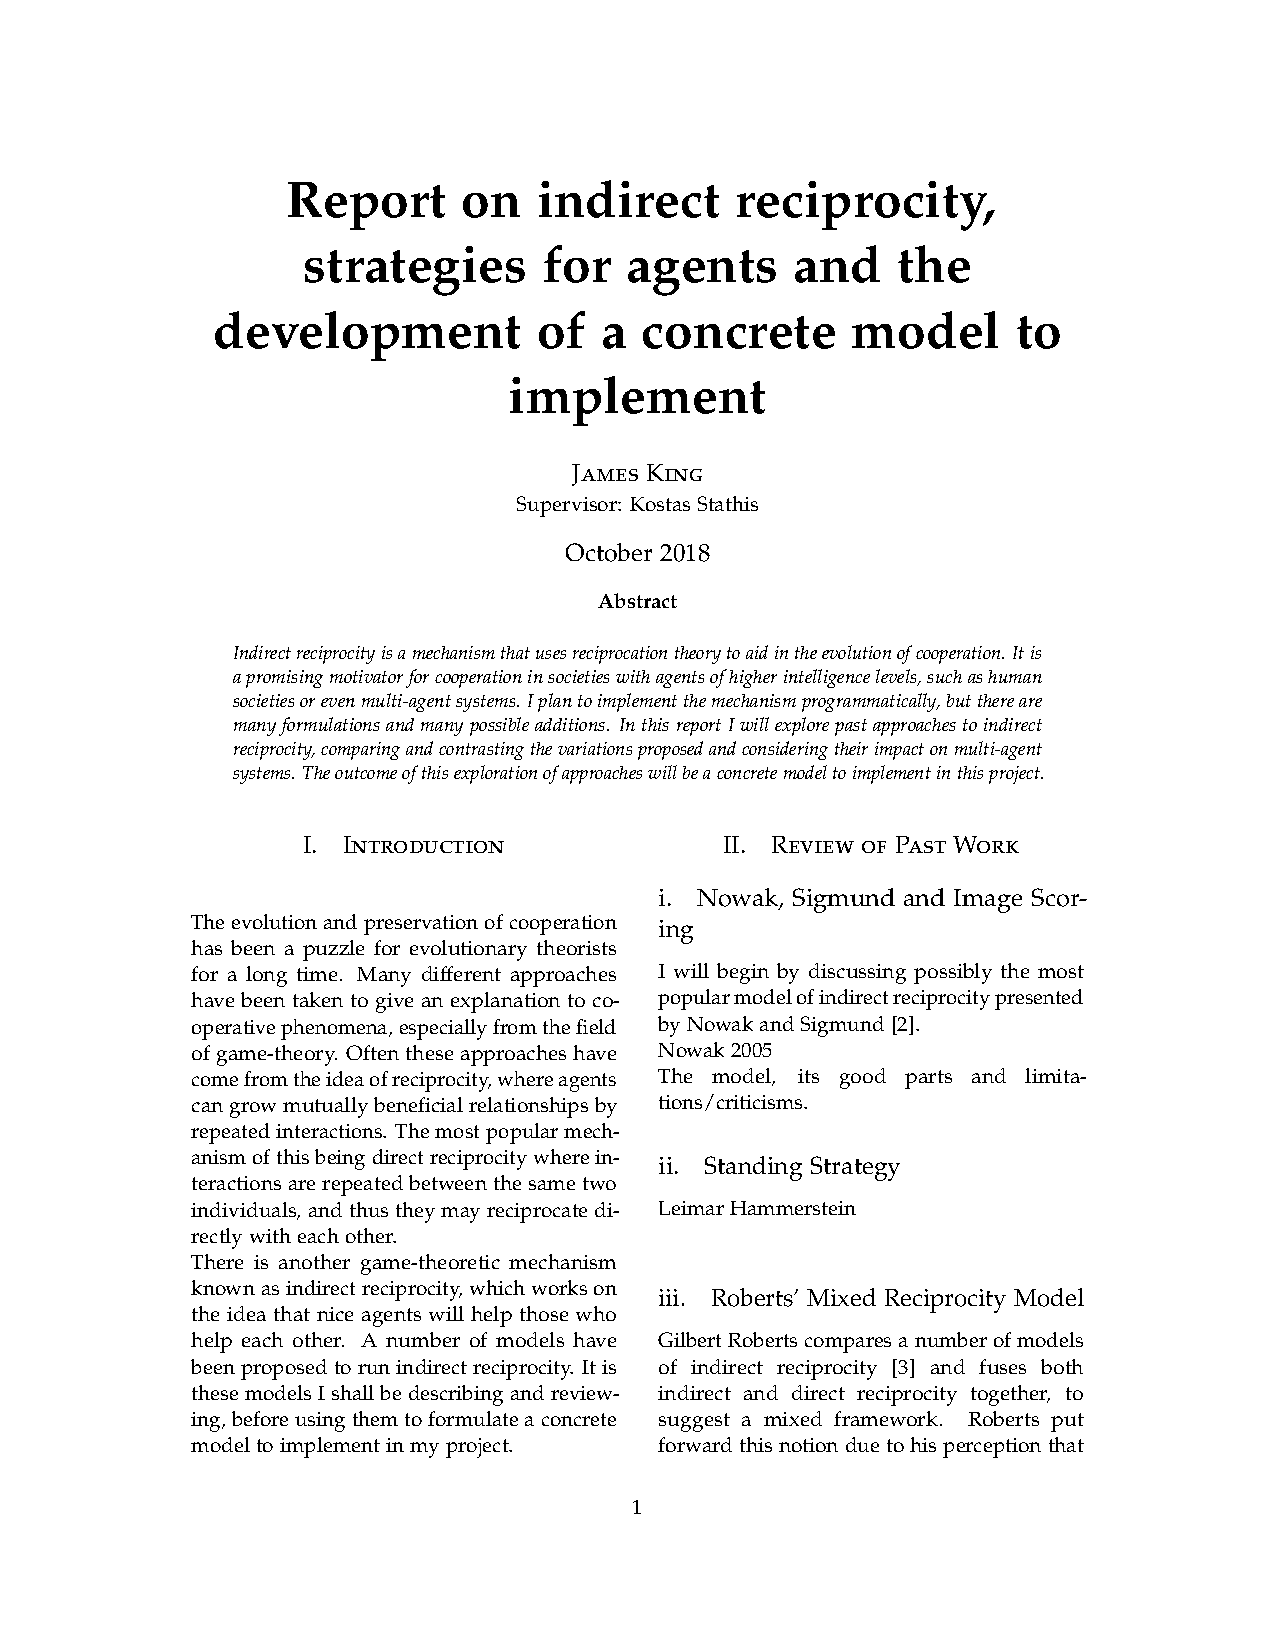
\includepdf[pages=-]{../../IndirRec/IndirRec.pdf}

\chapter{Diary}

\end{document}

\end{article}
